\section{Related Work}
With TensorRT, the latency of the NRX of Cammerer et al.~\cite{cammerer2023neural} grows linearly with the number of iterations~\cite{wiesmayr2025realtime}. Site-specific fine-tuning lets a two-iteration receiver outperform an untuned eight-iteration receiver on over-the-air recordings at two indoor sites~\cite{baytekin2026site}, but it requires recorded site data and degrades performance on the original training distribution~\cite{wiesmayr2025realtime}. Other work reduces per-slot compute or model size through dynamic depth, low-rank adapters, quantization, lighter attention or blocks, and model-driven hybrids~\cite{yang2022dynamic,vanbolderik2024layerskip,vanbolderik2024mean,vanbolderik2026loren,yellapragada2026qat,yellapragada2026axial,kawai2025unified,fan2025choose,gupta2025lowcomplexity,gansekoele2025rpe,honkala2026eqdeeprx,abdollahpour2025mdx}, some at a cost in accuracy. Yet all of these methods process each slot from scratch, which Kawai and Koodli~\cite{kawai2025unified} name as a limitation.

Pooling pilots across time is an established way to improve channel estimates: Wiener filtering weights pilots by their time--frequency correlation~\cite{hoeher1997wiener}, Kalman tracking propagates an estimate and its error covariance~\cite{komninakis2002kalman}, and 5G NR Release~17 standardizes DMRS bundling over several PUSCH slots~\cite{3gpp38830,3gpp38214}, which requires a correlated channel and a continuous transmit phase. Their weights come from channel statistics or a channel model that a BS must estimate per user, and they stay the same when a user's channel changes. Learned predictors use recurrent, state-space and transformer models over past channel estimates~\cite{mattu2022deep,mohsin2025continual,luo2025cpmamba,lagona2026transformer,gizzini2021talstm} or set the parameters of a Kalman tracker~\cite{pratik2021hkf}, but target channel prediction or tracking, and none conditions a multi-user NRX on stored pilot history. Our filter instead fits its weights per user by least squares on the stored pilots, like an adaptive filter~\cite{haykin2002adaptive}, chooses on the current slot how many entries to use, and feeds an NRX; after a channel change, it stays ahead of a classical multi-slot estimator given each condition's statistics, which even falls 0.56\,dB behind its single-slot version.

Within learned receivers, earlier slots enter mainly through the weights: online schemes retrain on decoder-recovered labels, on symbol decisions, or when a drift test fires~\cite{fischer2022adaptive,finish2022symbol,uzlaner2025asynchronous}, or track a posterior over the weights~\cite{gusakov2026online}, and pay in label delay, compute, or error propagation~\cite{fischer2022adaptive,fan2025defined}. Time-averaged channel covariances~\cite{liu2026universal,wiesmayr2026impact} remain valid across scheduling gaps but do not supply the instantaneous channel. Kunde et al.~\cite{kunde2025transformers} show that a fixed-weight attention layer over past pilot pairs can represent the symbol posterior, but only with asymptotic theory and single-user, uncoded experiments.

% Fig. 1 belongs to the Receiver Design. It is defined here because a full-width figure appears at the top of
% the next page: the Receiver Design starts at the end of this page and refers to the figure there.
\begin{figure*}[t]
\centering
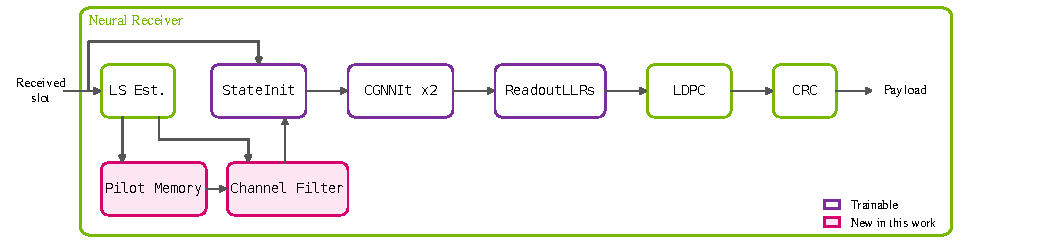
\includegraphics[width=\textwidth]{figures/receiver_architecture.pdf}
\caption{Proposed NRX for 5G NR PUSCH. The channel filter refines the LS estimate with the pilot memory before \texttt{StateInit}; its weights are fitted on the memory. The channel readout used only in training is not shown.}
\label{fig:architecture}
\end{figure*}

Despite these advances, no prior MU-MIMO NRX for 5G NR carries
channel estimates across slots to recover the accuracy lost to fewer
iterations. Unlike online adaptation, our receiver keeps its trained weights fixed and
stores only LS channel estimates, so it
needs no labels and no decoder feedback. Unlike DMRS bundling, it requires neither power
consistency nor phase continuity across the stored slots.
